\chapter {Interfacing a Thermistor}
\thispagestyle{empty}
\label{thermistor}

\newcommand{\LocTHERMfig}{\Origin/user-code/thermistor/figures}
\newcommand{\LocTHERMscicode}{\Origin/user-code/thermistor/scilab}
\newcommand{\LocTHERMscibrief}[1]{{\tt \seqsplit{%
        Origin/user-code/thermistor/scilab/#1}}, see \fnrefp{fn:file-loc}}
\newcommand{\LocTHERMardcode}{\Origin/user-code/thermistor/arduino}
\newcommand{\LocTHERMardbrief}[1]{{\tt \seqsplit{%
        Origin/user-code/thermistor/arduino/#1}}, see \fnrefp{fn:file-loc}}

%%%%%%%%%%%python starts
\newcommand{\LocTHERMpycode}{\Origin/user-code/thermistor/python}
\newcommand{\LocTHERMpybrief}[1]{{\tt \seqsplit{%
        Origin/user-code/thermistor/python/#1}}, see \fnrefp{fn:file-loc}}
%%%%%%%%%%%python ends

%%%%%%%%%julia
\newcommand{\LocTHERMjuliacode}{\Origin/user-code/thermistor/julia}
\newcommand{\LocTHERMjuliabrief}[1]{{\tt \seqsplit{%
        Origin/user-code/thermistor/julia/#1}}, see \fnrefp{fn:file-loc}}
%%%%%%julia

%%%%%%%%%OpenModelica starts
\newcommand{\LocTHERMOpenModelicacode}{\Origin/user-code/thermistor/OpenModelica}
\newcommand{\LocTHERMOpenModelicabrief}[1]{{\tt \seqsplit{%
        Origin/user-code/thermistor/OpenModelica/#1}}, see \fnrefp{fn:file-loc}}
%%%%%%OpenModelica ends

A thermistor, usually made of semiconductors or metallic oxides, is a
temperature dependent/sensitive resistor. Depending on the temperature
in the vicinity of the thermistor, its resistance changes. Thermistors
are available in two types, NTC and PTC. NTC stands for Negative
Temperature Coefficient and PTC for Positive Temperature
Coefficient. In NTC thermistors, the resistance decreases with the
increase in temperature and vice versa. Whereas, for PTC types, the
resistance increases with an increase in temperature and vice
versa. The temperature ranges, typically, from $-55^{\circ}$ Celsius
to $+125^{\circ}$ Celsius.

Thermistors are available in a variety of shapes such as beads, rods,
flakes, and discs. Due to their compact size and low cost, they are
widely used in the applications where even imprecise temperature
sensing is sufficient. They, however, suffer from noise and hence need
noise compensation. In this chapter we shall interface a thermistor
with the \arduino\ board.

\section{Preliminaries}
A typical thermistor and its symbolic representation are shown in
\ref{fig:therm} and \ref{fig:thermsym} respectively. The thermistor is
available on the shield provided with the kit.  It is a bead type
thermistor having a resistance of 10k at room temperature. A voltage
divider network is formed using thermistor and another fixed 10k
resistor. A voltage of 5 volts is applied across the series
combination of the thermistor and the fixed 10k resistor. Voltage
across the fixed resistor is sensed and is given to the ADC via pin
4. Hence at room temperature, both the resistors offer 10k resistance
resulting in dividing the 5V equally. A buzzer is also connected on
pin 3 which is a digital output pin.
Connections for this experiment are shown in \ref{fig:therm-conn}
and \ref{fig:buzzer-conn}.  Nevertheless, the user doesn't need to
connect any wire or component explicitly.


\begin{figure}
  \centering
  \subfloat[Pictorial representation of a thermistor\cite{therm-wiki}]{
    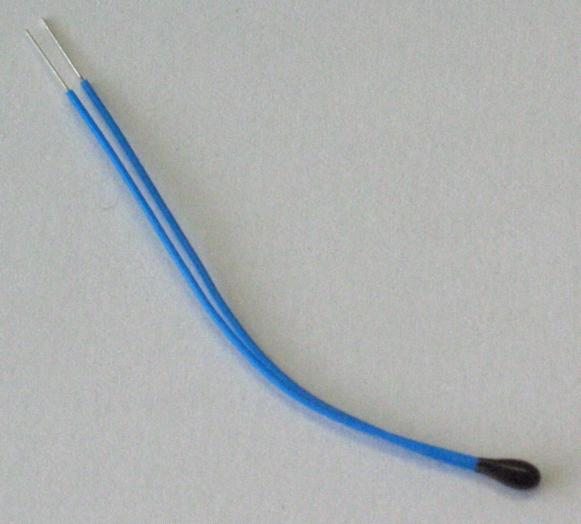
\includegraphics[width=\smfig]{\LocTHERMfig/NTC-bead.jpg}
    \label{fig:therm}} \hfill
  \subfloat[Symbolic representation of a thermistor]{
    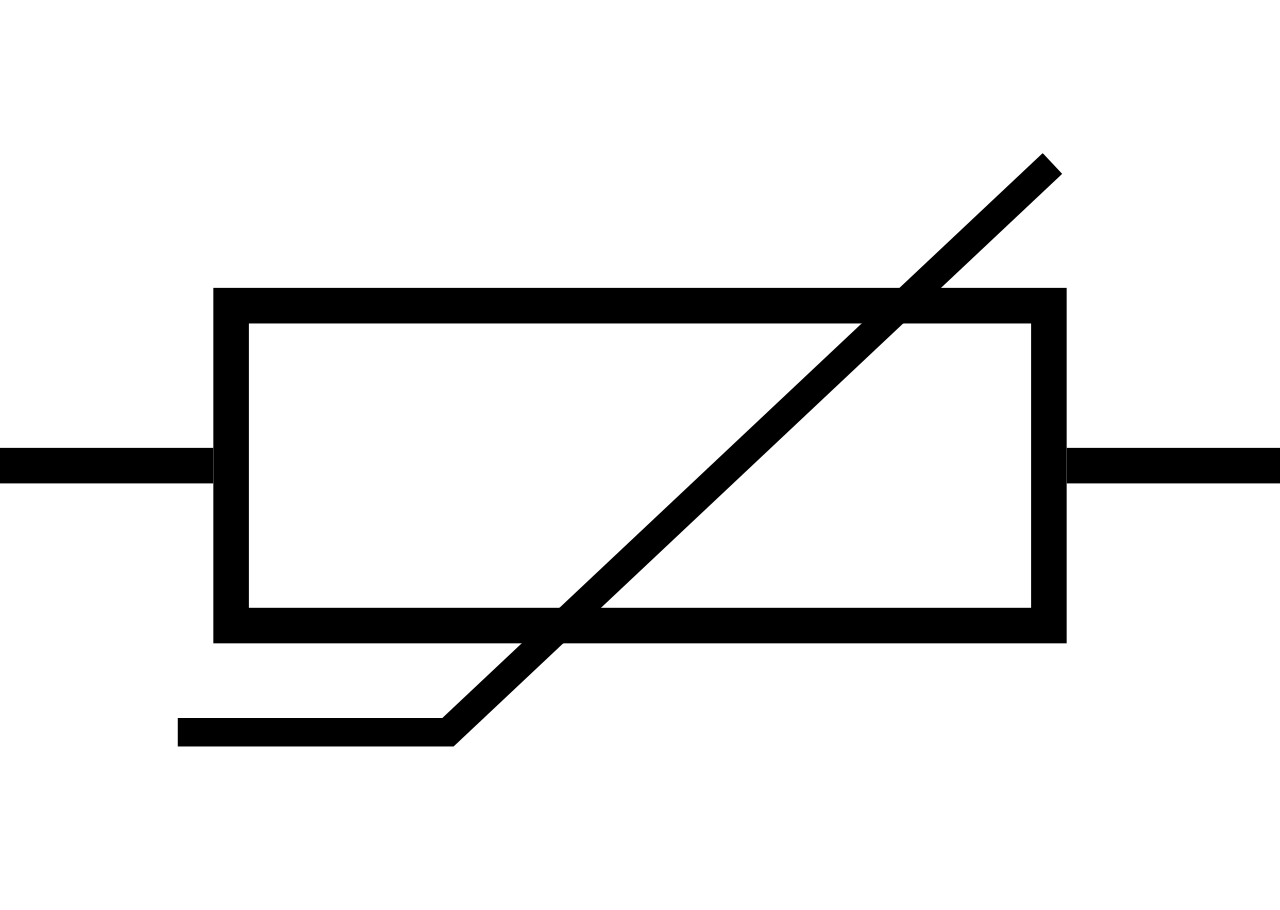
\includegraphics[width=\tnfig]{\LocTHERMfig/therm-sym.png}
    \label{fig:thermsym}}
  \caption{Pictorial and symbolic representation of a thermistor}
\end{figure}


\begin{figure}
  \centering
  \subfloat[Thermistor connection diagram]{
    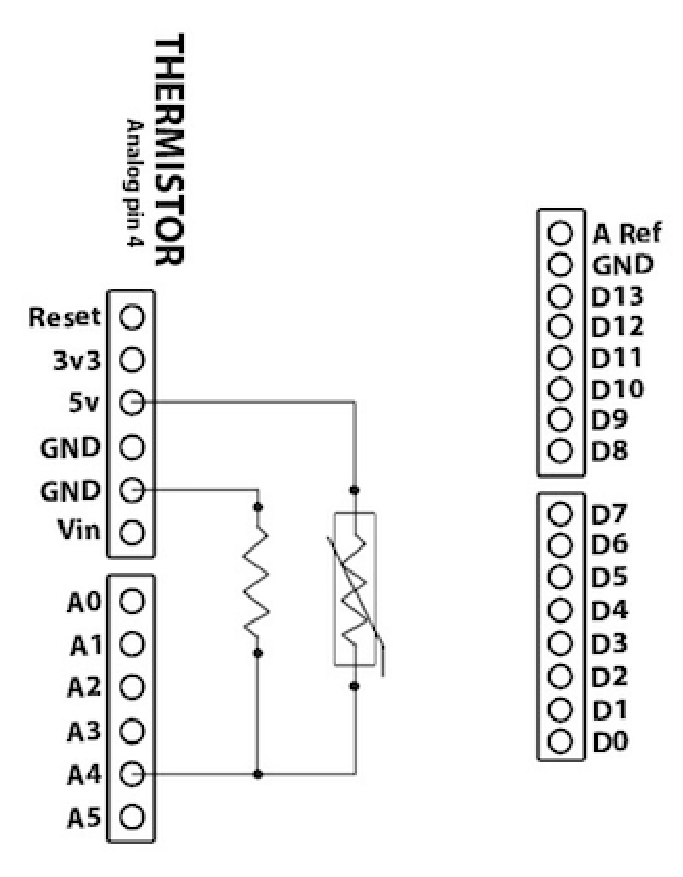
\includegraphics[width=\smfig]
    {\LocTHERMfig/THERMISTOR-Diagram-crop.pdf}
    \label{fig:therm-conn}} \hfill
  \subfloat[Buzzer connection diagram]{
    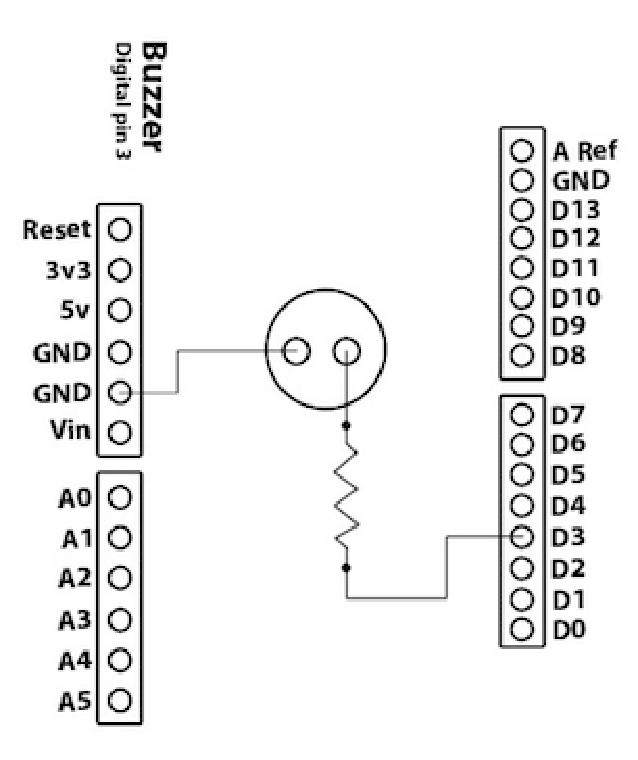
\includegraphics[width=\smfig]
    {\LocTHERMfig/BUZZER-Diagram-crop.pdf}
    \label{fig:buzzer-conn}}
  \caption{Internal connection diagrams for thermistor and buzzer on the shield}
\end{figure}

\section{Connecting a thermistor with \arduino\ using a breadboard}
This section is useful for those who either don't have a shield or don't want to use the shield
for performing the experiments given in this chapter.

A breadboard is a device for holding the components of a circuit and connecting
them together. We can build an electronic circuit on a breadboard without doing any
soldering. To know more about the breadboard and other electronic components,
one should watch the Spoken Tutorials on Arduino as published on
  {\tt https://spoken-tutorial.org/}. Ideally, one should go through all the
tutorials labeled as Basic. However, we strongly recommend the readers should
watch the fifth and sixth tutorials, i.e., {\tt First Arduino Program} and
  {\tt Arduino with Tricolor LED and Push button}.

In case you have a thermistor, and you want to connect it with \arduino\ on a breadboard,
please refer to \figref{fig:ard-therm-bread}. The connections given in this figure
can be used to read values from the thermistor connected to analog pin 4 on \arduino\
board.
\begin{figure}
  \centering
  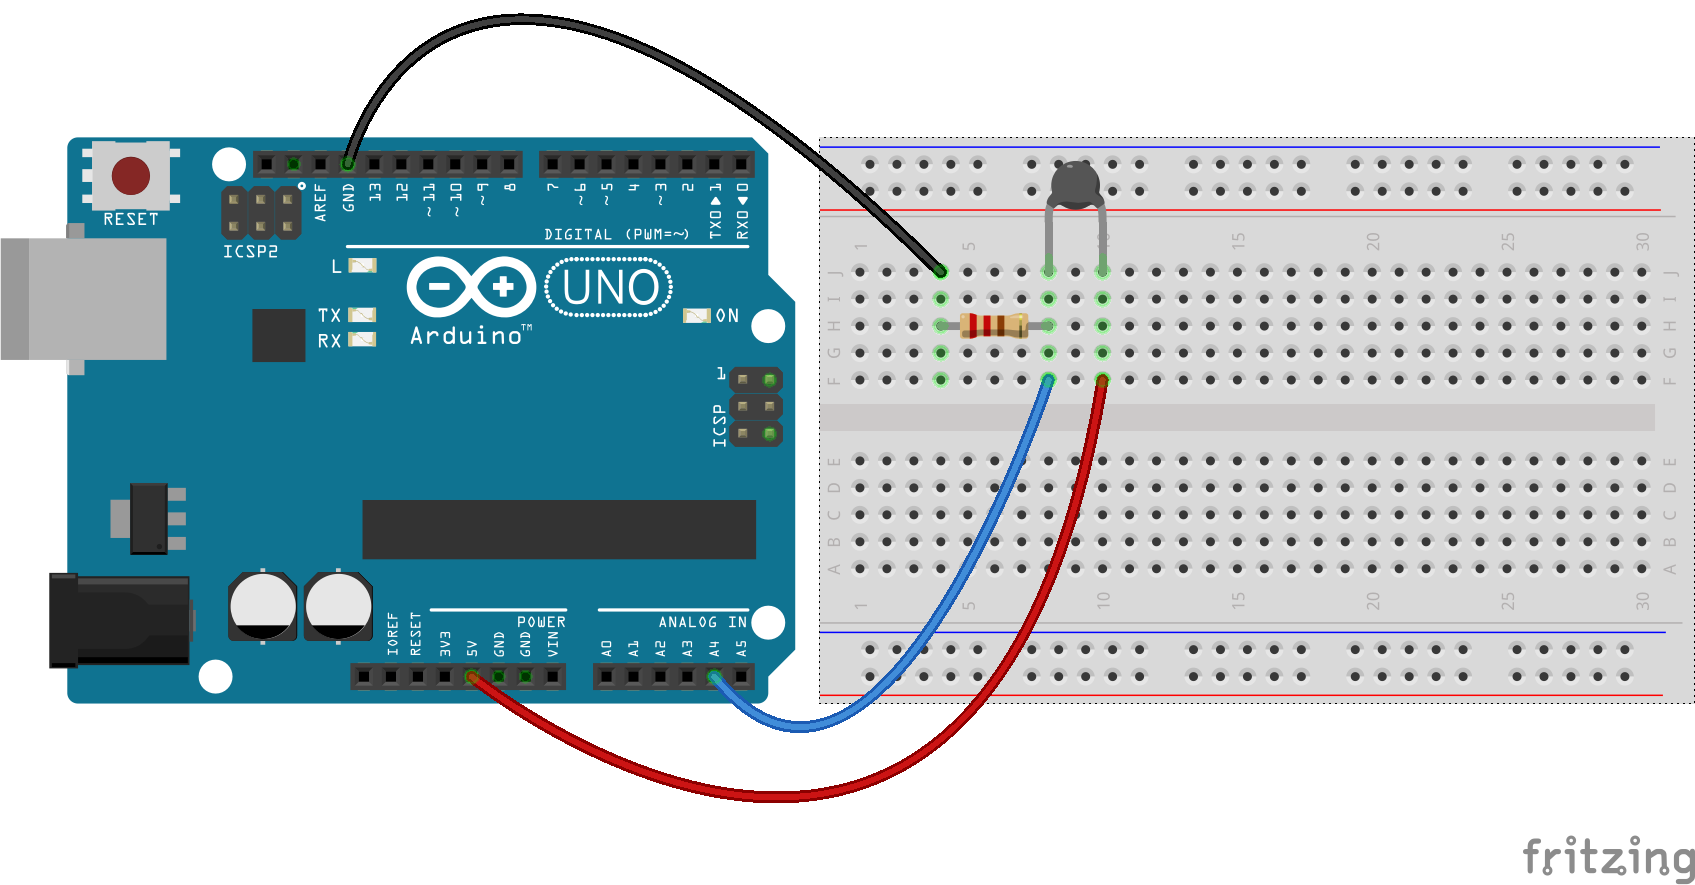
\includegraphics[width=\textwidth]{\LocTHERMfig/thermistor.png}
  \caption{A thermistor to read its values with Arduino Uno using a breadboard}
  %\redcolor{connected on pin no. D12}}
  \label{fig:ard-therm-bread}
\end{figure}
As shown in \figref{fig:ard-therm-bread}, one leg of the thermistor is connected
to 5V on \arduino\ and the other leg to the analog pin 4 on  \arduino. A resistor is also
connected to the same leg and grounded. From \figref{fig:therm-conn} and \figref{fig:ard-therm-bread}, one can infer that a resistor
along with the thermistor is used to create a voltage divider circuit. The varying
resistance of the thermistor is converted to a varying voltage. Finally, this voltage is used
by the analog pin 4 of \arduino\ in its logic.

\begin{figure}
  \centering
  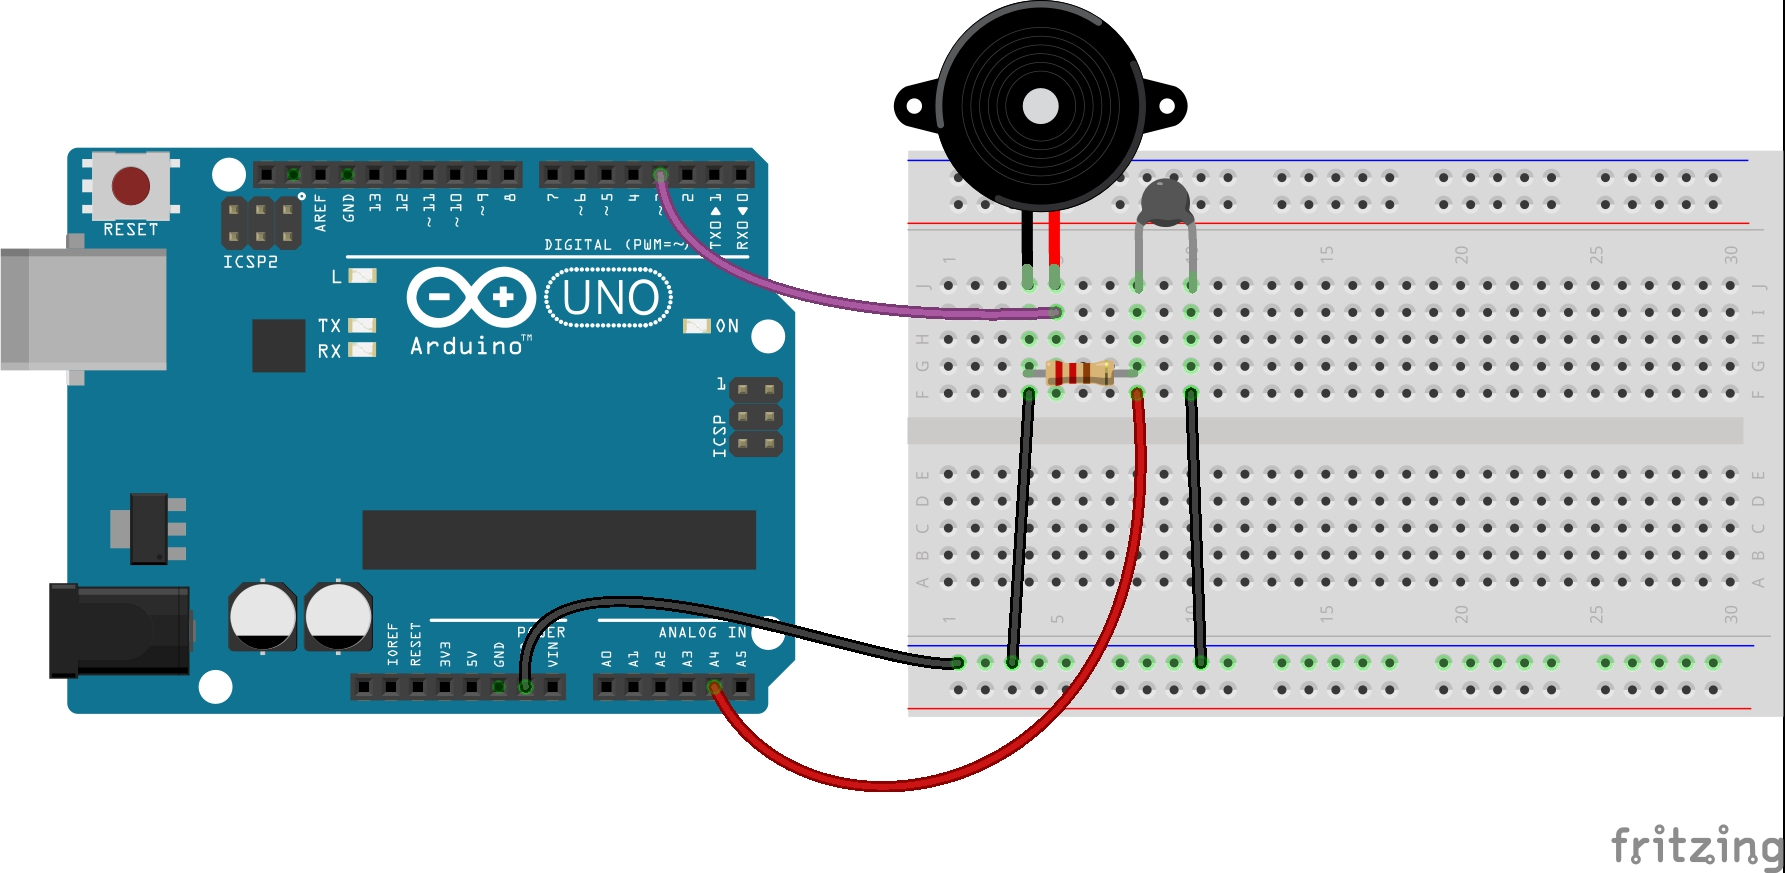
\includegraphics[width=\textwidth]{\LocTHERMfig/thermistor-buzzer-dark-color-wires.jpg}
  \caption{A thermistor to control a buzzer with Arduino Uno using a breadboard}
  %\redcolor{connected on pin no. D12}}
  \label{fig:ard-therm-buzzer}
\end{figure}
The connections shown in \figref{fig:ard-therm-buzzer} can be used to control a buzzer,
depending on the values from the thermistor. As shown in \figref{fig:ard-therm-buzzer},
digital pin 3 on \arduino\ is connected to the one of the legs of the buzzer. Another
leg of the buzzer is connected to GND of \arduino.


\section{Interfacing the thermistor from the Arduino IDE}
\subsection{Interfacing the thermistor}
In this section we will learn how to read values from the thermistor
connected at pin 4 of the \arduino\ board. We shall also see how to
drive a buzzer depending upon the thermistor values. The shield has to be attached to the \arduino\ board
before doing these experiments and the \arduino\ needs to be connected to the computer
with a USB cable, as shown in \figref{arduino}. The reader should go through the
instructions given in \secref{sec:ard-start} before getting started.

\begin{enumerate}
  \item A simple code to read the values from thermistor is given in
        \ardref{ard:therm-read}. The Arduino IDE based command for the analog read functionality is given by.
        \lstinputlisting[firstline=9,lastline=9]{\LocTHERMardcode/therm-read/therm-read.ino}
        where {\tt A4} represents the analog pin 4 to be read.
        The read value is stored in variable {\tt val} and is
        displayed using \lstinputlisting[firstline=10,lastline=10]{\LocTHERMardcode/therm-read/therm-read.ino}
        The command on next line

        \lstinputlisting[firstline=11,lastline=11]  {\LocTHERMardcode/therm-read/therm-read.ino}
        is used to put a delay of 500 milliseconds. This is to avoid very fast display of the read values. The entire reading and display operation is carried out 40 times.

        The values can be observed over the {\tt Serial Monitor} of Arduino IDE.
        The numbers displayed range from 0 to 1023. At room temperature you may get the
        output of ADC around 500. If a heating or cooling source is available,
        one can observe the increase or decrease in the ADC output. Although
        the thermistor is of NTC type, the ADC output increases with increase
        in temperature. This is because the voltage across the fixed resistor
        is sensed.

        While running this experiment,
        the readers should try holding (or rubbing) the thermistor with their fingertips.
        Doing so will transfer heat from the person holding the
        thermistor, thereby raising the temperature of the thermistor. Accordingly, they should observe the change in the thermistor values
        on the {\tt Serial Monitor}.

  \item In this experiment, we will turn the buzzer on depending
        on the temperature sensed by the thermistor. This experiment
        can be considered as a simple fire alarm circuit that
        detects fires based on a sudden change in temperature and
        activates the buzzer.

        The program for this is
        available at \ardref{ard:therm-buzzer}. We shall use the ADC output
        to carry this out. The buzzer is connected to pin 3, which is a
        digital output pin. The ADC output value is displayed on the serial
        monitor. At the same time, it is compared with a user-defined
        threshold, which has been set as 550 in this experiment. One may note that
        this threshold would vary according to the location and time of performing
        this experiment. Accordingly, the readers are advised to change this threshold
        in \ardref{ard:therm-buzzer}. For testing purposes, one may note the
        normal thermistor readings generated from the execution of \ardref{ard:therm-read}
        and set a threshold that is approximately 10 more than these readings.

        In this experiment, as soon as the ADC output exceeds 550, the buzzer is given a digital
        high signal, turning it on. The following lines of code perform this
        comparison and sending a {HIGH} signal to digital pin 3 on \arduino:
        \lstinputlisting[firstline=14,lastline=21]{\LocTHERMardcode/therm-buzzer/therm-buzzer.ino}
        A delay of half a second is introduced
        before the next value is read. While running this experiment,
        the readers should try holding (or rubbing) the thermistor with their fingertips.
        Doing so will transfer heat from the person holding the
        thermistor, thereby raising the temperature of the thermistor.
        Accordingly, they should observe whether the threshold of 550 is achieved
        and the buzzer is enabled.

        \paragraph{Note:} Once the thermistor value reaches 550 (the threshold), the value will remain the same
        (unless it is cooled). Therefore, the buzzer will continuously produce the sound, which might be
        a bit annoying. To get rid of this, the readers are advised to
        execute some other code on \arduino\ like \ardref{ard:therm-read}.

\end{enumerate}

\begin{exercise}
  Carry out the following exercise:
  \begin{enumerate}
    \item Put the thermistor in the vicinity of an Ice bowl. Take care not
          to wet the shield while doing so. Note down the ADC output value for
          0$^{\circ}$Celsius.
  \end{enumerate}
\end{exercise}

\subsection{Arduino Code}
\label{sec:therm-arduino-code}
\addtocontents{ard}{\protect\addvspace{\codclr}}

\begin{ardcode}
  \acaption{Read and display the thermistor values} {Read and display
    the thermistor values.  Available at
    \LocTHERMardbrief{therm-read/therm-read.ino}.}
  \label{ard:therm-read}
  \lstinputlisting{\LocTHERMardcode/therm-read/therm-read.ino}
\end{ardcode}

\begin{ardcode}
  \acaption{Turning the buzzer on using thermistor values}
  {Turning the buzzer on using the thermistor values read by
    ADC.  Available at
    \LocTHERMardbrief{therm-buzzer/therm-buzzer.ino}.}
  \label{ard:therm-buzzer}
  \lstinputlisting{\LocTHERMardcode/therm-buzzer/therm-buzzer.ino}
\end{ardcode}

